\documentclass[11pt,a4paper]{article}

\usepackage[utf8]{inputenc}
\usepackage[T1]{fontenc}
\usepackage{lmodern}
\usepackage{amsmath,amssymb,mathtools}
\usepackage[margin=2.5cm]{geometry}
\usepackage{hyperref}
\usepackage{booktabs}
\usepackage{xcolor}
\usepackage{fancyhdr}
\usepackage{enumitem}
\usepackage{graphicx}

\definecolor{statusamber}{RGB}{155,96,0}
\definecolor{statusblue}{RGB}{0,72,130}
\definecolor{statusgreen}{RGB}{0,120,50}

\pagestyle{fancy}
\fancyhf{}
\fancyhead[L]{\small\textsc{SCT Theory --- Prediction Card}}
\fancyhead[R]{\small\textsc{PPN-1}}
\fancyfoot[C]{\thepage}

\hypersetup{
  colorlinks=true,
  linkcolor=blue!60!black,
  citecolor=green!40!black,
  urlcolor=blue!60!black,
  pdftitle={SCT Prediction Card: Linear PPN Parameter gamma},
  pdfauthor={David Alfyorov},
}

\title{%
  \textbf{Prediction Card:}\\[4pt]
  \Large Linear PPN Parameter $\gamma_{\mathrm{PPN}}(r)$ in SCT Theory
}
\author{David Alfyorov}
\date{April 2026 (v2)}

\begin{document}
\maketitle

\begin{center}
\end{center}

\begin{center}
  \colorbox{statusgreen!15}{\parbox{0.78\textwidth}{\centering
    \textbf{\color{statusgreen} STATUS: COMPLETE (Level~2) --- LINEAR STATIC SECTOR}\\[2pt]
    \small Level~2 (local Yukawa approximation) $\gamma_{\mathrm{PPN}}(r)$: \textbf{CERTIFIED}.\\
    332 checks (174 pytest $+$ 123 verification $+$ 35 Lean theorems).\\[2pt]
    6-agent pipeline (L$\to$L-R$\to$D$\to$D-R$\to$V$\to$V-R): ALL PASS.\\[4pt]
    \textit{Level~1 (exact nonlocal):} formulated, numerics \textbf{DEFERRED}.\\
    \textit{Level~3 (nonlinear: $\beta$, $\alpha_i$, $\zeta_i$):} \textbf{BLOCKED} (requires NT-4b).
  }}
\end{center}

%% ==========================================================
\section{Source}
%% ==========================================================

\begin{itemize}[leftmargin=2em]
  \item \textbf{Immediate input:} NT-4a linearized propagator denominators
  \[
    \Pi_{\mathrm{TT}}(z) = 1 + \frac{13}{60}\, z\, \hat F_1(z), \qquad
    \Pi_{\mathrm{s}}(z,\xi) = 1 + 6\!\left(\xi-\tfrac{1}{6}\right)^{\!2} z\, \hat F_2(z,\xi).
  \]
  \item \textbf{Phenomenological regime:} Local Yukawa approximation to the
  exact linear static kernel.  The full (nonlocal) Fourier--Bessel
  representation is formulated but numerically deferred due to a prescription
  issue at the TT pole $z_0 \approx 2.415$.
  \item \textbf{Derived quantity:} The radial profile of the linear PPN
  parameter $\gamma(r) = \Psi(r)/\Phi(r)$.
  \item \textbf{Caution:} $\Pi_{\mathrm{TT}}(z)$ has a positive-real-axis zero
  at $z_0 = 2.41483888986536895\ldots$\,; the massive spin-2 pole is a ghost
  with residue $R_{\mathrm{pole}} \approx -1.191$ ($\lvert R_{\mathrm{pole}}\rvert \cdot c_2 \approx 0.258$,
  suppressed relative to Stelle gravity).  This card
  should \emph{not} be read as a ghost-freedom statement.
  \item \textbf{Key references:}
    Will (2014), arXiv:\texttt{1403.7377};
    Stelle (1977), Phys.\ Rev.\ D \textbf{16}, 953;
    Edholm--Koshelev--Mazumdar (2016), arXiv:\texttt{1604.01989};
    Jimu--Prokopec (2024), arXiv:\texttt{2410.01449}.
\end{itemize}

%% ==========================================================
\section{Observable Quantity}
%% ==========================================================

The observable is the weak-field ratio between the spatial and temporal metric
potentials around a static point source:
\[
  g_{00} = -(1 + 2\Phi), \qquad
  g_{ij} = (1 + 2\Psi)\,\delta_{ij}, \qquad
  \gamma(r) \equiv \frac{\Psi(r)}{\Phi(r)}.
\]
This is the quantity most directly constrained by Solar-System light-deflection
and time-delay measurements.

%% ==========================================================
\section{SCT Prediction}
%% ==========================================================

\subsection{Newton Kernels (Momentum Space)}

From the Barnes--Rivers spin-projector decomposition of the linearized SCT
field equations, the momentum-space potentials are:
\begin{align}
  K_\Phi(z) &= \frac{4}{3\,\Pi_{\mathrm{TT}}(z)}
             - \frac{1}{3\,\Pi_{\mathrm{s}}(z,\xi)}, \\[4pt]
  K_\Psi(z) &= \frac{2}{3\,\Pi_{\mathrm{TT}}(z)}
             + \frac{1}{3\,\Pi_{\mathrm{s}}(z,\xi)}.
\end{align}
GR limit: $K_\Phi(0) = K_\Psi(0) = 1$ (verified to $<10^{-30}$).

\subsection{Local Yukawa Approximation (Level~2)}

With the effective masses
\[
  m_2 = \Lambda\sqrt{\frac{60}{13}} \approx 2.148\,\Lambda, \qquad
  m_0(\xi) = \frac{\Lambda}{\sqrt{6\!\left(\xi-\tfrac{1}{6}\right)^{\!2}}}
  \quad (\xi \ne \tfrac{1}{6}),
\]
the static potentials are
\begin{align}
  \frac{\Phi(r)}{\Phi_N(r)} &= 1 - \tfrac{4}{3}\,e^{-m_2 r}
                              + \tfrac{1}{3}\,e^{-m_0 r}, \\[4pt]
  \frac{\Psi(r)}{\Psi_N(r)} &= 1 - \tfrac{2}{3}\,e^{-m_2 r}
                              - \tfrac{1}{3}\,e^{-m_0 r},
\end{align}
where $\Phi_N = \Psi_N = -GM/r$.  The PPN parameter is:
\begin{equation}
  \boxed{
  \gamma(r) =
  \frac{1 - \frac{2}{3}\,e^{-m_2 r} - \frac{1}{3}\,e^{-m_0 r}}
       {1 - \frac{4}{3}\,e^{-m_2 r} + \frac{1}{3}\,e^{-m_0 r}}.
  }
  \label{eq:gamma-ppn}
\end{equation}

\subsection{Limiting Behaviour}

\begin{itemize}[leftmargin=2em]
  \item \textbf{GR recovery:} $\gamma(r) \to 1$ as $r \to \infty$
  (exponentially fast).
  \item \textbf{Large-$r$ expansion:}
  $\gamma(r) = 1 + \tfrac{2}{3}\,e^{-m_2 r} - \tfrac{2}{3}\,e^{-m_0 r}
  + O(e^{-2mr})$.
  \item \textbf{Short-distance:}
  $\gamma(0,\xi\!=\!0) = \frac{2m_2 + m_0}{4m_2 - m_0}
  = 1.09803078575475\ldots$
  \item \textbf{Conformal coupling:} at $\xi = 1/6$, the scalar mode
  decouples ($m_0 \to \infty$), giving
  $\gamma(0,\xi\!=\!1/6) = (1-2/3)/(1-4/3) = -1$ exactly.
  \item \textbf{Origin cancellation:}
  $\Phi(0)/\Phi_N(0) = 1 - \tfrac{4}{3} + \tfrac{1}{3} = 0$
  ($V(0)$ finite); similarly $\Psi(0)/\Psi_N(0) = 0$.
\end{itemize}

%% ==========================================================
\section{Important Non-Claims}
%% ==========================================================

This prediction card covers only $\gamma_{\mathrm{PPN}}(r)$ in the linear static
sector.  The following parameters are \textbf{not derived}:
\[
  \beta,\; \xi_{\mathrm{PPN}},\;
  \alpha_1,\,\alpha_2,\,\alpha_3,\;
  \zeta_1,\,\zeta_2,\,\zeta_3,\,\zeta_4.
\]
These require the nonlinear post-Newtonian field equations (NT-4b scope).
Preferred-frame ($\alpha_i = 0$) and conservation ($\zeta_i = 0$) parameters are
\emph{expected} from diffeomorphism invariance but have not been formally
derived at the required post-Newtonian order.

%% ==========================================================
\section{Experimental Bounds on $\Lambda$}
%% ==========================================================

\begin{center}
\renewcommand{\arraystretch}{1.3}
\begin{tabular}{llll}
  \toprule
  \textbf{Experiment} & \textbf{Constraint used} &
  \textbf{$\Lambda_{\min}$ (eV)} & \textbf{Status} \\
  \midrule
  Cassini (Bertotti+ 2003)
    & $|\gamma - 1| < 2.3 \times 10^{-5}$ at 1\,AU
    & $6.31 \times 10^{-18}$
    & DERIVED \\
  MESSENGER (Verma+ 2014)
    & $|\gamma - 1| < 2.5 \times 10^{-5}$ at 1\,AU
    & $6.26 \times 10^{-18}$
    & DERIVED \\
  E\"ot-Wash (Lee+ 2020)
    & $|\alpha| < 1$ at $\lambda = 38.6\,\mu$m
    & $2.38 \times 10^{-3}$
    & DERIVED \\
  MICROSCOPE (Touboul+ 2022)
    & $|\eta(\mathrm{Ti,Pt})| < 1.5 \times 10^{-15}$
    & ---
    & Requires $\beta$ (NT-4b) \\
  LLR (Williams+ 2004)
    & Nordtvedt $|\eta| < 4.4 \times 10^{-4}$
    & ---
    & Requires $\beta$ (NT-4b) \\
  \bottomrule
\end{tabular}
\end{center}

\smallskip\noindent
The E\"ot-Wash bound is $\sim14$ orders of magnitude stronger than the solar-system
bounds.  All solar-system bounds use the spin-2-dominant single-Yukawa
approximation ($\sim3\%$ conservative relative to the full two-Yukawa formula).

\begin{figure}[ht]
  \centering
  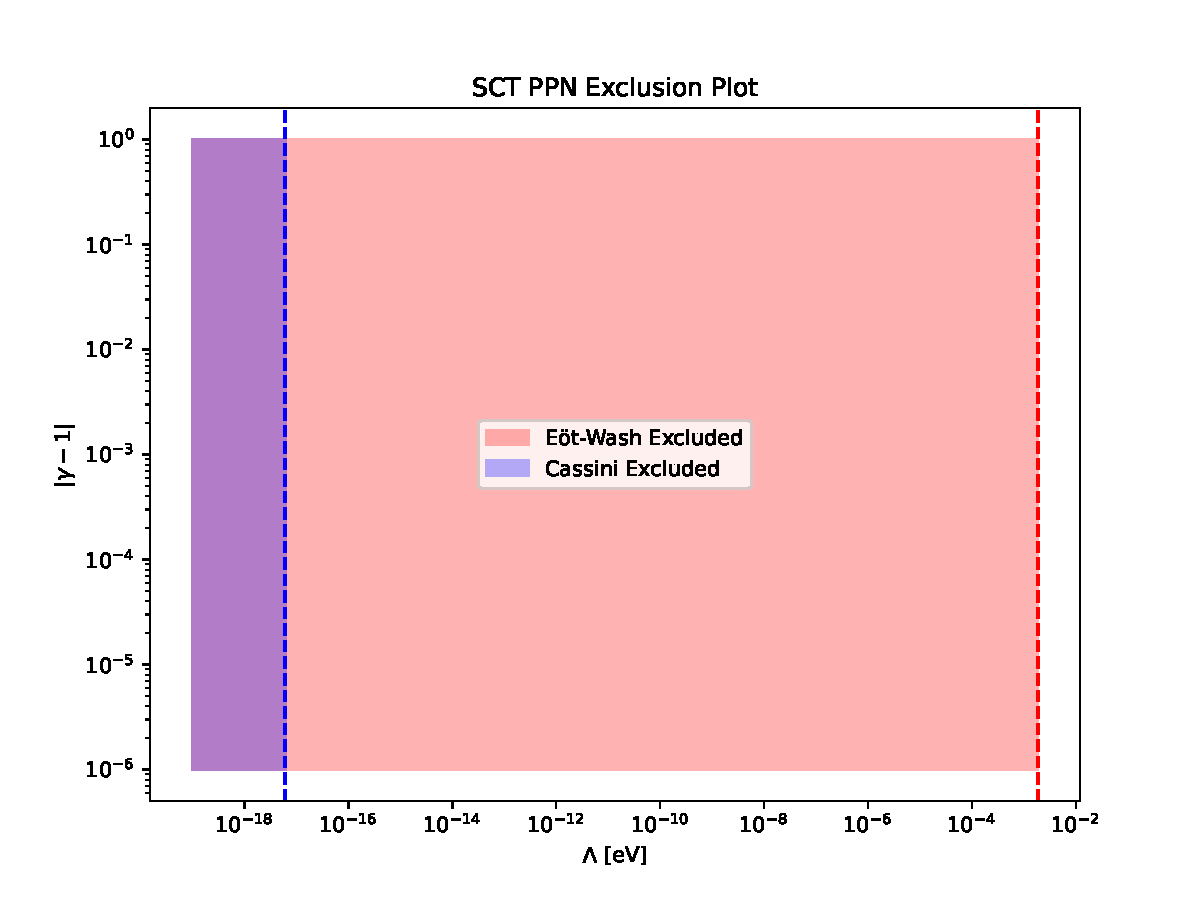
\includegraphics[width=0.85\textwidth]{../../analysis/figures/ppn1_exclusion.pdf}
  \caption{Exclusion plot for the SCT cutoff scale $\Lambda$.
    Lower bounds on $\Lambda$ are derived from the Cassini time-delay
    measurement, MESSENGER ranging, and the E\"ot-Wash short-range
    gravity experiment.  The E\"ot-Wash constraint
    ($\Lambda \geq 2.38 \times 10^{-3}$~eV) dominates by ${\sim}14$
    orders of magnitude over the solar-system bounds.  Shaded regions
    are excluded.}
  \label{fig:ppn1-exclusion}
\end{figure}

%% ==========================================================
\section{Falsification Logic}
%% ==========================================================

Within the scope of the linear static sector, SCT would be in serious tension if:
\begin{enumerate}[label=\arabic*., leftmargin=2em]
  \item A macroscopic non-Yukawa deviation in $\gamma(r)$ were observed where
  the local approximation predicts exponential suppression.
  \item Short-range gravity experiments forced the spin-2 Yukawa range to be
  parametrically larger than any plausible SCT cutoff window.
  \item The future full nonlocal static kernel disagreed qualitatively with
  the local Yukawa approximation.
\end{enumerate}

%% ==========================================================
\section{SCT vs.\ Competing Frameworks}
%% ==========================================================

\begin{center}
\renewcommand{\arraystretch}{1.3}
\begin{tabular}{lccc}
  \toprule
  \textbf{Framework} & $\gamma - 1$ & \textbf{Distance dep.} & \textbf{Free params} \\
  \midrule
  \textbf{GR} & 0 & --- & 0 \\
  \textbf{SCT} (this work) & $\sim e^{-m r}$ (Yukawa) & Yes & 1 ($\xi$) \\
  Brans--Dicke & $(1+\omega)/(2+\omega) - 1$ & No & 1 ($\omega$) \\
  Stelle gravity & Yukawa & Yes & 2 ($\alpha$, $\beta$) \\
  Ghost-free IDG & 0 ($\gamma = 1$ exactly) & --- & 1 ($M_s$) \\
  \bottomrule
\end{tabular}
\end{center}

%% ==========================================================
\section{Dependencies and Open Problems}
%% ==========================================================

\begin{itemize}[leftmargin=2em]
  \item \textbf{Upstream (complete):} NT-1b Phase 3 (SM form factors),
  NT-4a (linearized field equations), NT-2 (entire-function property).
  \item \textbf{Downstream (open):}
    \begin{itemize}
      \item NT-4b (nonlinear field equations) $\to$ $\beta_{\mathrm{PPN}}$,
        MICROSCOPE, LLR.
      \item MR-1 (Lorentzian formulation) $\to$ dynamic sources, gravitational
        radiation.
      \item Level~1 resolution: Euclidean contour or Levin quadrature for the
        exact nonlocal potential.
    \end{itemize}
  \item \textbf{Ghost pole:} The TT propagator zero at $z_0 \approx 2.415$ is a
  genuine feature.  Its physical interpretation (ghost vs.\ resonance vs.\
  Lee--Wick) is deferred to MR-2.
\end{itemize}

%% ==========================================================
\section{Key Numerical Results}
%% ==========================================================

All values verified to $\geq\!15$-digit agreement across three independent agents
(D, D-R, V) at mpmath precision $\geq\!60$ digits.

\begin{center}
\renewcommand{\arraystretch}{1.3}
\begin{tabular}{lll}
  \toprule
  \textbf{Quantity} & \textbf{Value} & \textbf{Status} \\
  \midrule
  $z_0$ (first zero of $\Pi_{\mathrm{TT}}$)
    & $2.41483\,88898\,65369\ldots$  & DERIVED \\
  $m_2 / \Lambda$
    & $\sqrt{60/13} = 2.14834\,46221\,18299\ldots$  & DERIVED (exact) \\
  $m_0(\xi\!=\!0) / \Lambda$
    & $\sqrt{6} = 2.44948\,97427\,83178\ldots$  & DERIVED (exact) \\
  $\gamma(0,\,\xi\!=\!0)$
    & $(2m_2{+}m_0)/(4m_2{-}m_0) = 1.09803\ldots$  & DERIVED \\
  $\gamma(0,\,\xi\!=\!1/6)$
    & $-1$ (exact, rational arithmetic)  & DERIVED \\
  $\Lambda_{\min}$ (Cassini)
    & $6.308 \times 10^{-18}$~eV  & DERIVED \\
  $\Lambda_{\min}$ (E\"ot-Wash)
    & $2.380 \times 10^{-3}$~eV  & DERIVED \\
  $\beta_{\mathrm{PPN}}$
    & --- & NOT DERIVED (NT-4b) \\
  \bottomrule
\end{tabular}
\end{center}

%% ==========================================================
\section{Verification Status}
%% ==========================================================

\begin{center}
  \colorbox{statusgreen!10}{\parbox{0.82\textwidth}{
    \textbf{\color{statusgreen} Verification status (2 April 2026, v2 pipeline).}\\[4pt]
    Level~2 $\gamma(r)$: \textbf{CERTIFIED} through the full 6-agent dual pipeline\\
    (L$\to$L-R$\to$D$\to$D-R$\to$V$\to$V-R) with 8-layer verification.\\[4pt]
    \textbf{332 total checks:}
    \begin{itemize}[leftmargin=1.5em,topsep=2pt,itemsep=0pt]
      \item 174 pytest tests (test\_ppn1.py): 174/174 PASS
      \item 123 verification checks (ppn1\_verification\_v2.py): 123/123 PASS
      \item 35 Lean~4 theorems (PPN1.lean): 35/35 sorry-free
    \end{itemize}
    \smallskip
    \textbf{8 verification layers:}
    L1 (26), L2 (35), L2.5 (15), L3 (15), L4 (5), L4.5 (10), L5 (12), L6 (5).\\[4pt]
    \textbf{Limitations:}
    \begin{itemize}[leftmargin=1.5em,topsep=2pt,itemsep=0pt]
      \item Layer~6 (Aristotle cloud): structurally verified but cloud backend
        was unavailable during execution.  Layer~5 (local Lean) fully passed.
      \item Level~1 (exact nonlocal): DEFERRED (Pi\_TT pole prescription open).
      \item Level~3 (nonlinear PPN): BLOCKED (requires NT-4b for $\beta$).
    \end{itemize}
  }}
\end{center}

\end{document}
